%%%%%%%%%%%%%%%%%%%%%%%%%%%%%%%%%%%%%%%%%%%%%%%%%%%%%%%%%%%%%%%%%%%%%%%%
% AAMAS 2027 Research Paper Track draft based on AAMAS_2027_sample.tex.
% The reported 900-second observations are audited. A separate prospective
% offline LLM controller has a documented one-shot generation receipt;
% the historical KNN and LinUCB rows are source-defined programmatic controls.
%%%%%%%%%%%%%%%%%%%%%%%%%%%%%%%%%%%%%%%%%%%%%%%%%%%%%%%%%%%%%%%%%%%%%%%%

\documentclass[sigconf,anonymous]{aamas}
\usepackage{booktabs}
\usepackage{placeins}
\graphicspath{{figures/}{../results/}{../results/figures/}}

% Official AAMAS 2027 copyright block (from AAMAS_2027_sample.tex).
\makeatletter
\gdef\@copyrightpermission{
  \begin{minipage}{0.2\columnwidth}
   \href{https://creativecommons.org/licenses/by/4.0/}{
\includegraphics[width=0.90\textwidth]{by}}
  \end{minipage}\hfill
  \begin{minipage}{0.8\columnwidth}
   \href{https://creativecommons.org/licenses/by/4.0/}{This work is licensed under a Creative Commons Attribution International 4.0 License.}
  \end{minipage}
  \vspace{5pt}
}
\makeatother

\setcopyright{ifaamas}
\acmConference[AAMAS 2027]{Proc.\@ of the 26th International Conference
on Autonomous Agents and Multiagent Systems (AAMAS 2027)}{3--7 May 2027}{Hanoi, Vietnam}{M.~Baldoni, F.~Fang, W.~Yeoh, N.~Yorke-Smith (eds.)}
\copyrightyear{2027}
\acmYear{2027}
\acmDOI{}
\acmISBN{}
\acmSubmissionID{TBD}
\submissionType{Research Paper Track}
\title[CIPHEUR: Structural Search Control]{CIPHEUR: LLM-Guided Structural Search Control for Conflict-Graph Optimization}

\begin{abstract}
Conflict-graph search can stagnate despite effective operators when interventions do not address current conflicts. Moreover, a disruptive intervention may appear unproductive before further search realizes its benefits. We study CIPHEUR, a structural search-control framework whose Structured Intervention Units (SIUs) connect conflict evidence to coordinated intervention and recovery. A common finite-plan interface supports programmatic selectors and online contextual decisions by a large language model (LLM). In the evaluated implementation, the programmatic experience-guided and value-guided selectors update from outcomes observed during a solve; the online LLM selects from the same plan registry while native optimization continues asynchronously. Both paths preserve the original objective and feasibility constraints. On eight constraint views of one satellite-ground scheduling contact source, each evaluated at five seeds and a 900-second budget, the online and two programmatic configurations exceed the CHILS-p4-custom mean objective by 0.336\%, 0.309\%, and 0.306\%, respectively. A separately frozen one-shot LLM-authored offline selector, CIPHEUR-off-GEN, returned legal plan IDs on 84 saved decision packets and averaged 1,136,347.357 contact-seconds across the 40-position frame (40/40 audited). The two programmatic controls are source-defined and are not attributed to that synthesis.
\end{abstract}

\keywords{large language models, maximum-weight independent set, search control, satellite-ground scheduling}
\ccsdesc[500]{Mathematics of computing~Combinatorial optimization}
\ccsdesc[300]{Computing methodologies~Search methodologies}

\begin{document}
\maketitle

\section{Introduction}

Effective combinatorial optimization depends on matching search actions to the opportunities available in the current state. Learning-assisted optimization and selection hyper-heuristics have made such decisions an explicit target of algorithm design~\cite{bengio2021methodological,drake2020selection}. Learning to schedule existing primal heuristics, for example, improves the allocation of search effort within a solver~\cite{chmiela2021schedule}. In conflict-graph optimization, this allocation also has a structural dimension: the value of an operation depends on the activities it displaces and the combinations it makes accessible. Exploiting this relationship calls for control decisions that connect observed conflicts to the subsequent course of search.

We study maximum-weight independent set (MWIS) optimization on resource-labelled conflict graphs. Weighted vertices represent candidate activities, and edges encode pairwise incompatibility. In satellite-ground scheduling, resource and temporal labels describe the conflicts among communication opportunities. Two search trajectories can attain similar objective values while excluding different combinations of activities, making the choice of intervention target consequential. A reconstruction can also reduce a trajectory's immediate value while creating opportunities for later improvement or exchange. These dependencies motivate the joint choice of \emph{how to intervene, where to act, and how search should continue}. The resulting control problem links structural targeting with the delayed effects of intervention.

Large language models (LLMs) offer complementary capabilities for addressing this problem. They can construct executable heuristics from problem descriptions and evaluative feedback~\cite{romeraparedes2024funsearch,liu2024eoh,ye2024reevo}, and make state-dependent heuristic choices during optimization~\cite{zhang2025laos,yang2025heuragenix}. Bringing these capabilities to conflict-graph search requires an actionable connection between contextual judgment and structural change. A useful decision must identify its target, organize the intervention and its continuation, and remain meaningful as the solver progresses. This motivates a common control abstraction through which executable policies and runtime reasoning can direct a continuing search.

We propose \textbf{CIPHEUR}, an LLM-guided structural search-control framework centered on the \textbf{Structured Intervention Unit (SIU)}. An SIU jointly specifies a structural target, an intervention, and the search behavior that follows it. Candidate SIUs are grounded in the conflicts affecting the current trajectories, linking each choice to a concrete search context. Subsequent choices use the solution-quality changes observed across executed intervention-recovery periods. Together, these elements establish a shared observation-decision-feedback loop in which each decision governs a coordinated course of search.

Two selection paths operate over this common SIU space. A programmatic path executes a controller constructed before deployment; its estimates may change as search produces new feedback. In the evaluated implementation, the experience-guided and contextual-value-guided paths are source-defined KNN and LinUCB selectors. An online LLM path chooses SIUs directly from current structural evidence and search history. The shared execution interface preserves the original objective and feasibility constraints, and the asynchronous online path lets native search proceed while the model responds. We separately froze one newly LLM-authored offline selector, CIPHEUR-off-GEN, from a recorded generation request. Its interface validation and matched 40-position result are reported here; it is distinct from the two source-defined controls.

The contributions of this study are threefold. \emph{First}, we formulate structure-grounded search control around SIUs that jointly express intervention, targeting, and recovery. \emph{Second}, we put source-defined programmatic selection and online LLM decisions over a shared executable control space, using feedback from actual search and asynchronous online execution. \emph{Third}, we report a matched 900-second evaluation on eight constraint views of one satellite-ground scheduling contact source, with five seeds per view. The three evaluated selectors have mean objectives 0.306--0.336\% above CHILS-p4-custom~\cite{grossmann2025chils} in this registered frame.

\section{Related Work}

\subsection{Independent-Set Search and Structural Guidance}

MWIS heuristics exploit solution structure to combine intensification with exploration. METAMIS uses efficient local moves and path relinking within a GRASP framework~\cite{dong2022metamis}, while CHILS combines iterated local search with cooperation based on differences among solutions~\cite{grossmann2025chils}. Learning-based graph optimization offers another form of structural guidance: Li et al.~\cite{li2018guided} use graph-convolutional predictions to guide tree search for independent sets. These approaches share the goal of using graph and solution information to expose promising combinations.

CIPHEUR studies this relationship at the level of search interventions. Resource-specific blocking evidence connects candidate activities to the trajectories that exclude them, providing a basis for choosing where to redirect search. A coordinated continuation then explores the opportunities created by the intervention. The emphasis is on converting structural evidence into decisions about the course of a population search, complementing work on local moves, solution exchange, and vertex-level guidance.

\subsection{Adaptive and Temporally Extended Search Control}

Selection hyper-heuristics adapt the use of low-level heuristics to search state and history~\cite{drake2020selection}; dynamic algorithm configuration learns policies for changing algorithm settings during execution~\cite{adriaensen2022dynamic}. Learned heuristic scheduling similarly allocates effort among existing solver components~\cite{chmiela2021schedule}. Adaptive large neighborhood search coordinates competing removal and insertion heuristics through performance feedback~\cite{ropke2006alns}, and learned neighborhood selection chooses variables for solver-based reoptimization~\cite{wu2021lns}. Together, these studies establish policy adaptation, effort allocation, and intervention targeting as complementary dimensions of search control.

Temporal abstraction provides a further dimension by treating an extended course of action as a decision unit, as formalized by the options framework~\cite{sutton1999options}. SIUs combine structural targeting with an explicit intervention-recovery sequence. A conflict anchor guides reconstruction priorities across the candidate activities, and the accompanying continuation specifies how the altered trajectory contributes to further search. Feedback summarizes quality changes over the executed sequence. This coupling makes the structural scope and observed effects of an intervention jointly available to the controller.

\subsection{LLM-Based Algorithm Design and Search Decisions}

LLM-based algorithm design couples program generation with empirical evaluation. FunSearch evolves executable programs using systematic scoring~\cite{romeraparedes2024funsearch}; EoH jointly evolves heuristic ideas and code~\cite{liu2024eoh}; and ReEvo uses reflective feedback to guide this search~\cite{ye2024reevo}. MCTS-AHD broadens exploration of heuristic programs through tree search~\cite{zheng2025mctsahd}, while EoH-S evolves complementary sets of heuristics~\cite{liu2026eohs}. This line of work demonstrates how LLM design knowledge can be retained in reusable algorithmic components.

A related line places model decisions within optimization. LAOS combines search-state information, operator credit, and replayed experience for adaptive operator selection~\cite{zhang2025laos}. LLMOA constructs sequences of low-level operators for continuous optimization~\cite{zhong2025llmoa}. HeurAgenix combines heuristic evolution with state-dependent selection, using Monte Carlo continuation estimates and supporting a fine-tuned lightweight selector~\cite{yang2025heuragenix}. These methods connect language-model capabilities with both algorithm construction and ongoing heuristic choice.

CIPHEUR makes the joint choice of target, intervention, and recovery the common task for programmatic selectors and an online LLM. Its SIU interface links control decisions to the conflicts observed during execution, while feedback reflects the search actually carried out. Asynchronous coordination lets online reasoning influence an evolving search through decisions whose structural meaning remains tied to their originating observations.

\section{Method Overview}

Given a weighted conflict graph $G=(V,E)$, CIPHEUR maintains feasible search trajectories and an incumbent independent set. At a decision point, the controller observes the current search state, recent execution history, and a finite registry of valid SIUs. A selected unit binds an operation to a trajectory and structural target and specifies the subsequent search steps. The native executor checks the selected plan against the current registry, installs it, and records interval outcomes for later decisions. The programmatic selectors and the online LLM differ in how they choose a plan; both use the same registered plan space and original graph objective. Details of plan construction, protected states, and native execution will be incorporated with the mechanism experiments.

\section{Experimental Results}

\subsection{Registered 900-Second Comparison}
% Generated by build_combined_table.py from the audited sources in combined_table_manifest.json.
\begin{table*}[t]
\centering
\footnotesize
\setlength{\tabcolsep}{3.5pt}
\caption{Audited 900\,s L002 objective ($10^3$ contact-seconds; higher is better), with overall Mean followed by eight views. Each method has 40 positions, five per view. $H_{340}$ abbreviates \texttt{g0340}, etc.; $M_{340/1200}$ abbreviates \texttt{gW0340\_gE1200\_s0150}, etc. AOC is 20--900\,s reference-gap area (\%; lower is better), available only for the three methods with recorded trajectories. GWMIN stopped before the cap; LS and LNS used independent process repeats because their binaries ignore the seed argument.}
\label{tab:c05-900s}
\begin{tabular}{@{}lrrrrrrrrrr@{}}
\toprule
Method & Mean & H$_{340}$ & H$_{680}$ & H$_{1200}$ & H$_{1800}$ & M$_{340/1200}$ & M$_{680/1200}$ & M$_{1200/340}$ & M$_{1200/680}$ & AOC$\downarrow$ \\
\midrule
\multicolumn{11}{@{}l}{\emph{Other methods}} \\
CHILS-p4-custom & 1,134.94 & 1,624.30 & 1,246.82 & 878.49 & 682.05 & 1,259.32 & 1,064.71 & 1,261.09 & 1,062.77 & --- \\
Feasibility Jump & 1,131.65 & 1,623.25 & 1,243.72 & 871.68 & 684.86 & 1,255.42 & 1,058.40 & 1,257.65 & 1,058.23 & --- \\
LS (StableSolver) & 1,131.31 & 1,611.34 & 1,239.05 & 884.04 & 680.69 & 1,255.74 & 1,061.96 & 1,256.32 & 1,061.31 & --- \\
LNS (StableSolver) & 1,125.48 & 1,606.76 & 1,233.78 & 876.86 & 680.51 & 1,248.57 & 1,054.24 & 1,248.35 & 1,054.78 & --- \\
FastWVC & 1,124.49 & 1,601.33 & 1,227.01 & 882.30 & 684.75 & 1,244.92 & 1,054.73 & 1,246.06 & 1,054.81 & --- \\
GRASP & 1,057.13 & 1,523.51 & 1,138.62 & 841.86 & 609.90 & 1,183.81 & 988.13 & 1,182.84 & 988.38 & --- \\
GWMIN & 991.62 & 1,428.00 & 1,065.57 & 809.27 & 489.40 & 1,130.38 & 940.99 & 1,125.63 & 943.71 & --- \\
\addlinespace[2pt]
\multicolumn{11}{@{}l}{\emph{CIPHEUR offline mode}} \\
CIPHEUR-off-EXP & 1,138.45 & 1,626.39 & 1,249.72 & 886.17 & 683.56 & 1,262.44 & 1,068.59 & 1,262.76 & 1,067.97 & 0.2418 \\
CIPHEUR-off-VAL & 1,138.42 & 1,626.42 & 1,249.67 & 884.79 & 683.64 & 1,262.72 & 1,068.73 & 1,263.57 & 1,067.79 & 0.2523 \\
CIPHEUR-off-GEN & 1,136.35 & 1,624.75 & 1,248.62 & 882.20 & 682.72 & 1,259.97 & 1,065.91 & 1,260.59 & 1,066.03 & --- \\
\addlinespace[2pt]
\multicolumn{11}{@{}l}{\emph{CIPHEUR online mode}} \\
CIPHEUR-online & 1,138.76 & 1,627.02 & 1,249.81 & 885.94 & 683.85 & 1,263.30 & 1,068.55 & 1,263.77 & 1,067.86 & 0.2406 \\
\bottomrule
\end{tabular}
\end{table*}


The registered comparison uses eight constraint views of the single physical contact source \texttt{CP-SCALE-AU-L002}. Each view is run with seeds 67, 71, 73, 79, and 83 under a 900-second wall-clock budget. Every position uses a population of four and one native solver thread. The four arms are CIPHEUR-online, CIPHEUR-off-EXP, CIPHEUR-off-VAL, and CHILS-p4-custom; all 160 arm--graph--seed results passed the independent identity, input-hash, objective, and feasibility audit. The source-defined experience-guided and value-guided controls implement KNN and LinUCB selection, respectively. Here \textit{off} means that the selector uses no runtime LLM call; the available records do not attribute these programs to LLM synthesis. The reported mean gives each of the eight views equal weight after averaging its five seeds.

Across the 40 matched graph--seed positions, CIPHEUR-online has a higher
final objective than CHILS-p4-custom in all 40. It exceeds CIPHEUR-off-EXP
and CIPHEUR-off-VAL in 24 positions each, and is below each in the
remaining 16. No pair has an equal final objective.

% Append verified experiment fragments in completion order. Empty source files
% are intentional hooks and can be replaced without changing this main file.
% Additional completed 900-second baselines from the adjacent verified comparison.
% Independent local audit evidence:
% experiments/classical_wmis_grasp_900s_6workers_v2_20261009/independent_audit.json
% experiments/stablesolver_gwmin_900s_6workers_full40_timed_20261009/analysis_local/audit.json
% experiments/published_cloud_download_20261009/local_independent_audit/fj/audit.json
% experiments/published_cloud_download_20261009/local_independent_audit/fastwvc/audit.json
% experiments/cipheur_siu_20261009/classical_crosscheck/lns_second_independent_crosscheck.json
% experiments/cipheur_siu_20261009/classical_crosscheck/ls_second_independent_crosscheck.json
\subsection{Additional Completed External Baselines}

Six additional methods in Table~\ref{tab:c05-900s} have independently
audited feasible results on all eight L002 views.
Each reported mean is over 40 executions, five per view, under a 900-second
cap. GWMIN terminated before the cap on every position. The official LS and
LNS binaries ignore their seed arguments, so their five positions per view
are fresh process repeats. LNS used a 890-second native limit inside the
900-second outer cap and measured 891.1--892.5\,s wall time. The LS command
requested 850\,s native time; its reported native times were 854.2--872.6\,s,
and measured outer wall times were 856.8--874.4\,s.

\subsection{Framework-Level SIU Ablation}
The primary framework ablation compares the complete online configuration
with two controls on matched graph--seed--host positions. \emph{SIU-Off}
keeps the initial \texttt{v05\_nonllm\_adaptive} native plan and makes no
subsequent SIU decisions or plan installations; the native plan retains
its original diversity-based search rule. \emph{Fixed-Spread}
retains the SIU execution interface and scheduled decision points, but
returns the same legal single-operation \texttt{spread} plan each time.
Both controls use the same 900\,s budget, four native trajectories, and
original objective and feasibility checks; neither calls a model during
deployment. Fixed-Spread also changes the mix of executed plans, so it is
a coarse no-adaptation control rather than a selector-only causal test.
The original four-view screen is retained as supplementary
selector and evidence controls. CIPHEUR-off-RAND is a random
programmatic selector that executes SIUs without deployment model calls
and therefore does not represent component removal.
\IfFileExists{../extension_8x5/analysis/core_siu_full_table.tex}{%
  \input{../extension_8x5/analysis/core_siu_full_summary.tex}%
  \input{../extension_8x5/analysis/core_siu_full_table.tex}%
  \input{../extension_8x5/analysis/core_siu_full_deltas.tex}%
}{%
  \IfFileExists{../extension_8x5/analysis/core_controls_full_table.tex}{%
    Both framework controls completed the full eight-view, five-seed frame (40/40 audited positions each). Their equal-view mean objectives in contact-seconds are SIU-Off 1,134,403.037 and Fixed-Spread 1,137,567.142.
%
    \begin{table*}[t]
\centering
\scriptsize
\setlength{\tabcolsep}{2.5pt}
\caption{Completed 900\,s eight-view framework controls. Objectives are in $10^3$ contact-seconds; each row contains 40 independently audited positions (five seeds per view). The matched CIPHEUR-online extension is reported separately when complete.}
\label{tab:core-controls-full}
\begin{tabular}{@{}lrrrrrrrrr@{}}
\toprule
Configuration & Mean & $H_{340}$ & $H_{680}$ & $H_{1200}$ & $H_{1800}$ & $M_{340/1200}$ & $M_{680/1200}$ & $M_{1200/340}$ & $M_{1200/680}$ \\
\midrule
SIU-Off (native adaptive) & 1,134.40 & 1,623.33 & 1,247.08 & 879.53 & 680.13 & 1,258.04 & 1,064.39 & 1,258.59 & 1,064.13 \\
Fixed-Spread & 1,137.57 & 1,625.51 & 1,249.32 & 884.17 & 682.96 & 1,261.49 & 1,067.76 & 1,262.54 & 1,066.78 \\
\bottomrule
\end{tabular}
\end{table*}
%
    Across the 12 audited matched positions, the mean objectives in contact-seconds are SIU-Off 1,205,338.566, Fixed-Spread 1,208,186.125, CIPHEUR-online 1,209,579.778. The paired differences in contact-seconds are CIPHEUR-online-minus-SIU-Off +4,241.212 (12/12 positive); CIPHEUR-online-minus-Fixed-Spread +1,393.654 (9/12 positive).
%
    \begin{figure}[t]
\centering
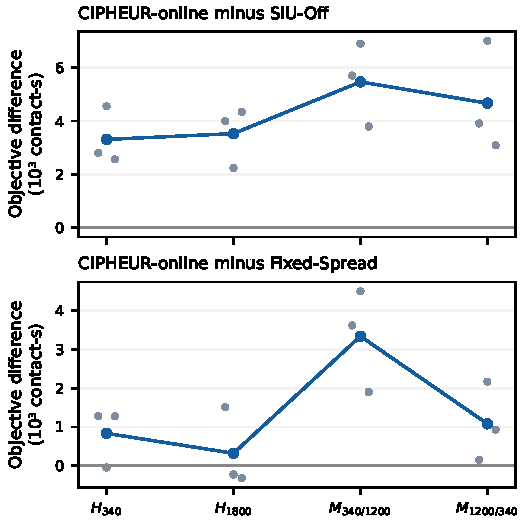
\includegraphics[width=\columnwidth]{../extension_8x5/analysis/core_siu_screen_deltas.pdf}
\Description{Two panels of paired CIPHEUR-online minus SIU-Off and CIPHEUR-online minus Fixed-Spread objective differences, with seed points and per-view means.}
\caption{Matched CIPHEUR-online-minus-control objective differences for the initial four-view screen. Dots are seeds; blue markers show per-view means. Positive values favor CIPHEUR-online.}
\label{fig:core-siu-screen}
\end{figure}
%
  }{%
    \IfFileExists{../extension_8x5/analysis/core_siu_screen_table.tex}{%
      Across the 12 audited matched positions, the mean objectives in contact-seconds are SIU-Off 1,205,338.566, Fixed-Spread 1,208,186.125, CIPHEUR-online 1,209,579.778. The paired differences in contact-seconds are CIPHEUR-online-minus-SIU-Off +4,241.212 (12/12 positive); CIPHEUR-online-minus-Fixed-Spread +1,393.654 (9/12 positive).
%
      \input{../extension_8x5/analysis/core_siu_screen_table.tex}%
      \begin{figure}[t]
\centering
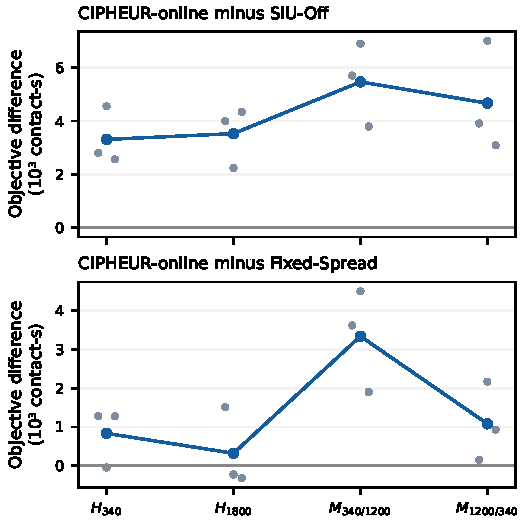
\includegraphics[width=\columnwidth]{../extension_8x5/analysis/core_siu_screen_deltas.pdf}
\Description{Two panels of paired CIPHEUR-online minus SIU-Off and CIPHEUR-online minus Fixed-Spread objective differences, with seed points and per-view means.}
\caption{Matched CIPHEUR-online-minus-control objective differences for the initial four-view screen. Dots are seeds; blue markers show per-view means. Positive values favor CIPHEUR-online.}
\label{fig:core-siu-screen}
\end{figure}
%
    }{}%
    \IfFileExists{../extension_8x5/analysis/siu_off_full_partial.tex}{%
      \input{../extension_8x5/analysis/siu_off_full_partial.tex}%
    }{}%
    \IfFileExists{../extension_8x5/analysis/fixed_spread_full_partial.tex}{%
      \input{../extension_8x5/analysis/fixed_spread_full_partial.tex}%
    }{}%
  }%
}

\subsection{Supplementary Four-View Control Screen}
CIPHEUR-off-RAND is a prespecified random programmatic selector
with no deployment model calls; we do not attribute its code to LLM
synthesis. It continues to execute SIUs and is not the SIU-Off arm.
No-Struct masks resource witnesses and plan contexts in the model request
while retaining the legal plan IDs and their executable bindings.
Across 12 matched positions, the paired CIPHEUR-online minus
CIPHEUR-off-RAND and CIPHEUR-online minus Single-Op
means are 538.377 and 93.655 contact-seconds
(6/12 and 8/12 positive), respectively. The paired CIPHEUR-online
minus No-Struct mean is 131.678 contact-seconds (8/12 positive). Single-Op installed
251/252 model proposals; one request returned HTTP 504. No-Struct received
252/252 model responses and installed 251/252 proposals; one response
failed plan validation. The 12 No-Struct positions passed the independent
graph-feasibility and integer-objective audit; all 252 submitted prompts
passed the masked-field audit.

\IfFileExists{../results/siu_ablation_table.tex}{\begin{table}[t]
\centering
\scriptsize
\setlength{\tabcolsep}{2.5pt}
\caption{Initial matched 900\,s L002 four-view screen: mean and per-view objectives in $10^3$ contact-seconds. Each completed row has 12 audited positions (three seeds per view). CIPHEUR-off-RAND retains SIU execution with stratified random selection; CIPHEUR-off-GEN follows a separate frozen offline protocol.}
\label{tab:siu-ablation-screen}
\begin{tabular}{@{}lrrrrr@{}}
\toprule
Configuration & Mean & $H_{340}$ & $H_{1800}$ & $M_{340/1200}$ & $M_{1200/340}$ \\
\midrule
Single-Op & 1,209.49 & 1,626.72 & 684.88 & 1,262.85 & 1,263.50 \\
No-Struct & 1,209.45 & 1,627.12 & 684.40 & 1,263.02 & 1,263.25 \\
CIPHEUR-off-RAND & 1,209.04 & 1,626.24 & 684.37 & 1,262.39 & 1,263.17 \\
CIPHEUR-off-GEN & 1,207.12 & 1,624.50 & 683.14 & 1,260.34 & 1,260.50 \\
CIPHEUR-online & 1,209.58 & 1,626.09 & 683.84 & 1,264.46 & 1,263.93 \\
\bottomrule
\end{tabular}
\end{table}
}{}
\IfFileExists{../results/siu_paired_deltas.tex}{\begin{figure}[t]
\centering
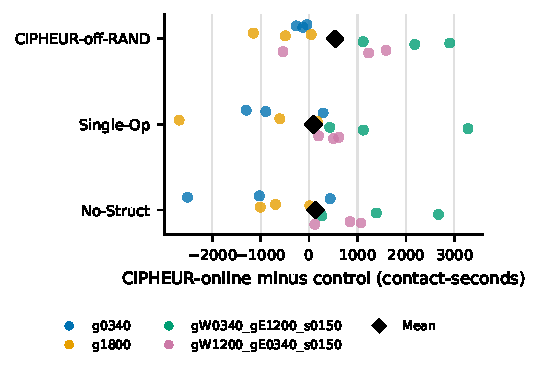
\includegraphics[width=\columnwidth]{../results/siu_paired_deltas.pdf}
\Description{Paired objective differences for CIPHEUR-off-RAND, Single-Op, and No-Struct across matched graph, seed, and host positions; points show runs and diamonds show configuration means.}
\caption{Paired 900\,s objective differences for matched graph, seed and server partition. Points are individual runs; diamonds are configuration means.}
\label{fig:siu-paired-deltas}
\end{figure}
}{}
% Generated from the audited C05 900-second private numeric logs.
% Compile from workspace root, or redefine \CIPHEURLogsDir before input.
\providecommand{\CIPHEURLogsDir}{figures/}
\subsection{Recorded Search Trajectories and Execution}
The final objectives and recorded 20--900\,s AOC values appear together in
Table~\ref{tab:c05-900s}.
\begin{figure*}[t]
\centering
\includegraphics[width=.86\textwidth]{\CIPHEURLogsDir on_off_anytime_relative.pdf}
\Description{Mean paired CIPHEUR-online minus CIPHEUR-off-EXP and CIPHEUR-off-VAL incumbent value, normalized by each view's best recorded terminal feasible value, over wall-clock time 20 to 900 seconds.}
\caption{Recorded anytime differences for CIPHEUR-online versus CIPHEUR-off-EXP and CIPHEUR-off-VAL. Values are paired by view and seed; positive values favor CIPHEUR-online. Each series averages 40 pairs. The step curves use saved epoch-end incumbent observations without interpolation.}
\label{fig:cipheur-log-anytime}
\end{figure*}
\begin{figure*}[t]
\centering
\includegraphics[width=.90\textwidth]{\CIPHEURLogsDir attainment_difference.pdf}
\Description{Two empirical attainment-difference heatmaps, CIPHEUR-online minus CIPHEUR-off-EXP and CIPHEUR-online minus CIPHEUR-off-VAL, on a fixed wall-clock and reference-gap target grid. Each cell uses 40 matched graph--seed positions.}
\caption{Empirical attainment differences for CIPHEUR-online versus the two recorded programmatic controls. Each cell reports the percentage-point difference in the fraction of 40 graph--seed positions reaching the stated reference-gap target by the stated wall-clock time; red favors CIPHEUR-online. The grid is unsmoothed. The view reference is the best audited terminal feasible value among the four registered arms.}
\label{fig:cipheur-log-attainment}
\end{figure*}
At 900\,s and a 0.05\% reference-gap target, 10/40 online runs attained the target, compared with 6/40 for off-EXP and 6/40 for off-VAL.
\begin{figure*}[t]
\centering
\includegraphics[width=.76\textwidth]{\CIPHEURLogsDir siu_event_aligned.pdf}
\Description{Event-aligned recorded incumbent change, mean search-trajectory change, and population diversity around installed directed-reseed entries.}
\caption{Observed directed-SIU execution. Of 406 directed intervals, 401 have an installed native directed-reseed entry. Each point averages events within a run, then averages runs. Positive times are retained only before plan replacement (401 events through 24 s; 400 at 30 s). These observational changes are not causal effects.}
\label{fig:cipheur-log-siu}
\end{figure*}
\begin{figure*}[t]
\centering
\includegraphics[width=.86\textwidth]{\CIPHEURLogsDir async_execution_timeline.pdf}
\Description{Recorded first 140 seconds of the first preregistered graph and seed: request pending and HTTP periods above native search epochs, with plan installations marked by triangles.}
\caption{Recorded asynchronous execution, CP-SCALE-AU-L002\_\_g0340, seed 67, first 140 wall-clock seconds. Pale upper bars denote request-to-receipt intervals, dark upper bars HTTP intervals, lower bars native work (orange for directed reconstruction), and triangles installed plans.}
\label{fig:cipheur-log-async}
\end{figure*}
\begin{table}[t]
\centering
\caption{Online request and native-work timing aggregated over the 40 recorded CIPHEUR-online runs. Intervals overlap and must not be added to solver wall time. Token usage was unavailable in the saved provider receipts.}
\label{tab:cipheur-log-overhead}
\begin{tabular}{@{}p{.65\columnwidth}r@{}}
\toprule
Measure & Recorded value \\
\midrule
Model calls / installed plans & 840 / 838 \\
Latency median / p90 (s) & 11.06 / 13.87 \\
Native work during pending (s) & 9837.4 \\
Pending time with native work (\%) & 99.9 \\
Native cycles while model pending & 2,720,049 \\
\bottomrule
\end{tabular}
\end{table}


% intervention_events results pending verified experiment output.

% async_execution results pending verified experiment output.

\IfFileExists{../sync_async/analysis/sync_async_results.tex}{\input{../sync_async/analysis/sync_async_results.tex}}{}
% Prospective generation record; the separately audited L002 result is
% included by ../offline_llm_c05/analysis_l002/results_l002.tex.
\subsection{Prospective Offline Controller Generation}

We generated one new executable selector, CIPHEUR-off-GEN, for the
shared SIU registry in a single offline Codex CLI request on October 9,
2026. The request specified
\texttt{gpt-6-luna} with low reasoning effort and required a deterministic
\texttt{select\_plan(packet, plans)} function that returns a current legal plan
ID. The first raw candidate was retained without objective-guided revision.
The separately written integration layer checks the returned ID before the
unchanged CIPHEUR executor installs the corresponding plan. This prospective
selector is distinct from the earlier source-defined KNN and LinUCB controls.

\begin{table}[t]
\centering
\small
\caption{Frozen generation and interface-validation record for the new offline LLM selector. Hashes are SHA-256 prefixes of the archived artifacts.}
\label{tab:offline-generation}
\begin{tabular}{@{}lp{0.58\columnwidth}@{}}
\toprule
Record & Value \\
\midrule
Generation & One request; \texttt{gpt-6-luna}, low effort \\
Exact prompt & \texttt{37cb63f4} \\
Raw response & \texttt{c667c0a7} \\
Frozen selector source & \texttt{8a9c0131} \\
Interface validation & 84/84 legal plan IDs on saved L002 seed-83 packets from four views; deterministic repeat and no input mutation \\
New-source use & No L003 graph or outcome used for generation or validation \\
\bottomrule
\end{tabular}
\end{table}

The authored selector was first audited on a separately registered
12-position L002 frame. Its extension to the remaining 28 positions follows
a second frozen protocol using the same selector source and paired host map.
The full L002 frame includes the four seed-83 positions used for interface
validation; validation checked plan-ID legality without revising the first
candidate against solver outcome scores.

\IfFileExists{../offline_llm_c05/analysis_l002_full/results_l002_full.tex}{%
  \subsection{Prospective CIPHEUR-off-GEN at 900 Seconds}
The frozen LLM-authored selector completed all 40 predeclared L002 positions across eight views and five seeds. All positions passed the independent graph-feasibility and integer-objective audits, and the selector made zero deployment LLM calls. Its equal-view mean is 1,136,347.357 contact-seconds.
%
}{%
  \IfFileExists{../offline_llm_c05/analysis_l002/results_l002.tex}{%
    \input{../offline_llm_c05/analysis_l002/results_l002.tex}%
  }{}%
}
\IfFileExists{../offline_llm_c05/analysis_l003/results_l003.tex}{\input{../offline_llm_c05/analysis_l003/results_l003.tex}}{}
% Independently audited 12/12 positions for each of 3 completed L003 arms.
% Author-provided L003 non-use attestation, not an independently complete development ledger.
\begingroup\raggedright
\noindent\textbf{CP-SCALE-L003 cross-source evaluation (900 s, contact seconds).}\par
\noindent The authors attest that the L003 source group was newly constructed and was not used for prompt design, code tuning, or controller selection. Source and graph hashes are independently checkable; the global non-use history is an author-provided statement. The archived off-EXP and off-VAL implementations are programmatic KNN and LinUCB controls, respectively.\par
\noindent CHILS-p4-custom: Mean 1,464,422.108; AU-H 1,623,289.585, AU-M 1,259,639.231, AP-H 1,690,811.593, AP-M 1,283,948.025.\par
\noindent CIPHEUR-off-EXP: Mean 1,467,303.722; AU-H 1,627,711.221, AU-M 1,264,049.745, AP-H 1,692,549.222, AP-M 1,284,904.699.\par
\noindent CIPHEUR-off-VAL: Mean 1,467,089.653; AU-H 1,627,468.221, AU-M 1,263,209.138, AP-H 1,692,805.837, AP-M 1,284,875.414.\par
\endgroup


% Add the official sample's balance package for final pagination if required.
\FloatBarrier
\bibliographystyle{ACM-Reference-Format}
\bibliography{CIPHEUR_references}
\end{document}
